%----------------------------------------------------------------------------   
\chapter{Architektúra}
%----------------------------------------------------------------------------

A Kubernetes architektúra tervezése során a fő szempont az volt, hogy teljes
mértékben úgy nézzen ki kívülről, mintha egy szimpla rtpengine lenne. De 
mögötte egy mikroszolgáltatásokból álló alkalmazás legyen, mely képes
az benne rejlő rtpengine-t megfelelően konfigurálni.

Ezt a fürtöt a BME által szolgáltatott szervereken építettem ki, mi szám szerint
4 szervert tartalmaz melyek az alábbi elrendezésben vannak összekötve.

\begin{figure}[!ht]
	\centering
	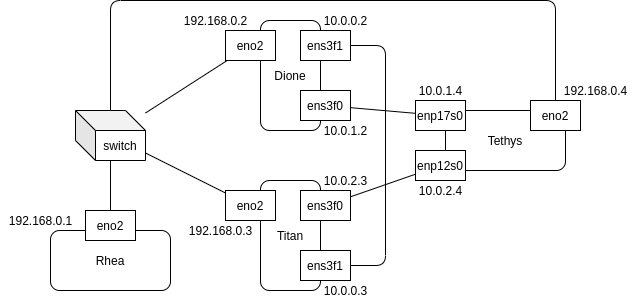
\includegraphics[width=1\textwidth, keepaspectratio]{figures/servers.png}
	\caption{Szerverek összeköttetése}
	\label{fig:HVSpaces}
\end{figure}

Az ábrán szereplő szervereket kettő részre lehet szétbontani, ahol az egyik
konkréten a Kubernetes fürt a másik pedig a forgalom generálására használatos.
Az előbbibe tartozik a Rhea, mint mester csomópont és dolgozó csomópontok közé 
a Dione és a Titan. Majd értelemszerűen az utóbbiba tartozik a Tethys. 

A szerverek között a kapcsolatot a vonalakkal jeleztem, melyek, mint látszik
sok esetben direkt összeköttetésben vannak egymással. Ez azért van, mert ezek
az interfészek 40 gigabitesek és az egyetemen nem állt rendelkezésre ilyen 
sebességű switch. Ezáltal a Kubernetes fürt telepítése során különös figyelmet
kellett szentelni annak, hogy ezek az interfészek helyesen legyenek felkonfigurálva.

De, mint látszik a hálózatban szerepel egy switch, amibe az eno2 interfészek vannak
becsatlakoztatva. Ezek az interfészek 1 gigabites sebességgel rendelkeznek, amik
a sok nagy sebességű forgalmat nem képes kiszolgálni, viszont még így is hasznosak
a hálózat szempontjából. Mivel a telepített Kubernetes fürt vezérlő- és adatsíkja
ezen a két összeköttetésen osztozik. Szóval a lassabb interfészeken kommunikál az
API szerver és a kubelet, míg a kube-proxy a nagy sebességű hálózati kártyákat 
használja. Így lehetett egy olyan magas határt szabni a lehetséges forgalom
sebességének, amibe nehéz beleütközni. 

Ahhoz, hogy az előzőleg leírt hálózat elkülönítés működjön a Kuberspray programot 
használtam, mert ennél könnyedén lehetett a telepítés során kettő különböző interfészt
beállítani. A kuberspray programmal Kubernetes fürtöket lehet telepíteni szimplán
szerverekre. A különlegessége az, hogy Ansible-t használ erre a célra. Szóval elég
a mester szerver számára lehetővé tenni, hogy működjön az ssh a többi szerverrel és
egyetlen konfigurációs fájl indításával képes minden szükséges szoftvert feltelepíteni
és azokat beállítani. Az Ansible-l nagyjából bármilyen folyamatot lehet automatizálni a
szerverek között. 

\section{Kubernetes architektúra}

A címben említett architektúra írja le, hogy a fürtön belül hogyan milyen Kubernetes
erőforrások találhatóak meg és azok, hogyan vannak egymással összekötve. A következő
ábrát kifejtve lehet ezt legjobban elmagyarázni.

\begin{figure}[!ht]
	\centering
	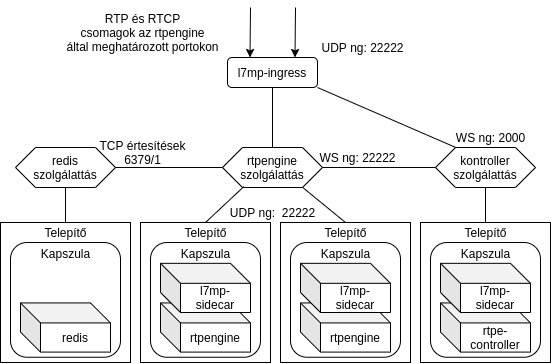
\includegraphics[width=1\textwidth, keepaspectratio]{figures/cluster.png}
	\caption{Fürt felépítése}
	\label{fig:HVSpaces}
\end{figure}

